\documentclass[english]{beamer}
\usepackage{makeidx}
\usepackage{color}
\usepackage{graphicx}
%\usepackage[pdftex]{graphicx}
\usetheme{Goettingen}
\setbeamercovered{transparent}

\usenavigationsymbolstemplate{}

\definecolor{ListingBorderColor}{gray}{0.55}
\definecolor{ListingBackgroundColor}{gray}{0.95}

\usepackage{babel}
\usepackage{hyperref}
\usepackage{enumerate}
\usepackage{enumerate}
\usepackage{longtable}
\usepackage[T1]{fontenc}
\usepackage{ucs}
\usepackage[latin1]{inputenc}
\usepackage{textcomp}
\usepackage{alltt}
\usepackage{listings}
\usepackage{fancyvrb}

\title{Git Basics}
\author[Sonia Hamilton, Bart Trojanowski]
{Bart Trojanowski \href{mailto:bart@jukie.net}{bart@jukie.net}\\
This edit {Sonia Hamilton \href{mailto:sonia@snowfrog.net}{sonia@snowfrog.net}}}
\institute{Jukie Networks Inc.}
\date{31st August, 2012}

\newcommand{\mysection}[2]{%
  \hypertarget{#2}{}%
  \section{#1}%
  \label{#2}%
}
\newcommand{\mysubsection}[2]{%
  \hypertarget{#2}{}%
  \subsection{#1}%
  \label{#2}%
}

\definecolor{code-black}{rgb}{0,0,0}
\definecolor{code-green}{rgb}{0,0.3,0}
\definecolor{code-orange}{rgb}{0.4,0.3,0}
\definecolor{code-blue}{rgb}{0,0,0.5}
\definecolor{code-red}{rgb}{0.7,0,0}
\definecolor{code-gray}{rgb}{0.7,0.7,0.7}
\definecolor{code-white}{rgb}{1,1,1}
\newcommand{\ttt}[1]{%
\texttt{\textcolor{code-black}{#1}}%
}
\newcommand{\CMD}[1]{%
\texttt{\textcolor{code-blue}{#1}}%
}
\newcommand{\cmd}[1]{%
\texttt{\textcolor{code-orange}{#1}}%
}
\newcommand{\gui}[1]{%
\texttt{\textcolor{code-green}{#1}}%
}
\newcommand{\err}[1]{%
\texttt{\textcolor{code-red}{#1}}%
}
\newcommand{\fnt}[1]{%
\texttt{\textcolor{code-gray}{#1}}%
}
\newcommand{\hide}[1]{%
\texttt{\textcolor{code-white}{#1}}%
}

\newcommand{\black}[1]{%
\textcolor{code-black}{#1}%
}
\newcommand{\faint}[1]{%
\textcolor{code-gray}{#1}%
}
\newcommand{\green}[1]{%
\textcolor{code-green}{#1}%
}
\newcommand{\blue}[1]{%
\textcolor{code-blue}{#1}%
}
\newcommand{\red}[1]{%
\textcolor{code-red}{#1}%
}

\begin{document}
% =====================================================================
\label{header}\hypertarget{header}{}
\frame{\maketitle}

% =====================================================================
% =====================================================================
\mysection{Concepts}{_concepts}
% =====================================================================
\mysubsection{Decentralized}{concepts:decentralized}

% ---------------------------------------------------------------------
\begin{frame}
	\frametitle{Intro}
\begin{itemize}
	\item breaks \\
	\item mobile phones \\
        \item questions \\
\end{itemize}
\end{frame}

% ---------------------------------------------------------------------
\begin{frame}
\frametitle{Centralized SCM - Subversion}
\includegraphics[width=\linewidth]{centralized.eps}
\begin{itemize}
        \item operations \textcolor{red}{require} server
                \begin{itemize}
                        \item single point of failure
                        \item bottleneck
                \end{itemize}
\end{itemize}
\end{frame}

% ---------------------------------------------------------------------
\begin{frame}
\frametitle{Decentralized SCM}

\includegraphics[width=\linewidth]{decentralized_single.eps}
\begin{itemize}
        \item you're your own server
\end{itemize}
\end{frame}

% ---------------------------------------------------------------------
\begin{frame}
\frametitle{Decentralized SCM}
\includegraphics[width=\linewidth]{decentralized.eps}
\begin{itemize}
        \item anyone can be a server
\end{itemize}
\end{frame}

% =====================================================================
\mysubsection{Structure}{concepts:structure}
% ---------------------------------------------------------------------
\begin{frame}
\frametitle{Structure}

\includegraphics[width=\linewidth]{struct-02.eps}
\vspace{\baselineskip}
\begin{center}
        the three 'areas'
\end{center}
\vspace{\textheight}
\end{frame}

% ---------------------------------------------------------------------
\begin{frame}
\frametitle{Structure}
\begin{columns}[t]
        \begin{column}[T]{.5\textwidth}
                directed acyclic graph

                \vspace{.1\textheight}
                ``DAG''
        \end{column}
        \begin{column}[T]{.5\textwidth}
                \includegraphics[width=\linewidth]{repo-dag.eps}
        \end{column}
\end{columns}

\end{frame}

% ---------------------------------------------------------------------
\begin{frame}
\frametitle{Structure}
\begin{columns}[t]
        \begin{column}[T]{.5\textwidth}
                References
                \begin{itemize}
                        \item tags
                \end{itemize}
        \end{column}
        \begin{column}[T]{.5\textwidth}
                \includegraphics[width=\linewidth]{repo-tags.eps}
        \end{column}
\end{columns}

\end{frame}

% ---------------------------------------------------------------------
\begin{frame}
\frametitle{Structure}
\begin{columns}[t]
        \begin{column}[T]{.5\textwidth}
                References
                \begin{itemize}
                        \item tags
                        \item branches
                \end{itemize}
        \end{column}
        \begin{column}[T]{.5\textwidth}
                \includegraphics[width=\linewidth]{repo-branches.eps}
        \end{column}
\end{columns}

\end{frame}

% ---------------------------------------------------------------------
\begin{frame}
\frametitle{Structure}
\begin{columns}[t]
        \begin{column}[T]{.5\textwidth}
                HEAD
                \begin{itemize}
                        \item current checkout
                        \item points to branch
                \end{itemize}
        \end{column}
        \begin{column}[T]{.5\textwidth}
                \includegraphics[width=\linewidth]{repo-head.eps}
        \end{column}
\end{columns}

\end{frame}

% ---------------------------------------------------------------------
\begin{frame}
\frametitle{Structure}
\begin{columns}[t]
        \begin{column}[T]{.5\textwidth}
                HEAD
                \begin{itemize}
                        \item current checkout
                        \item points to branch
                        \item sometimes detached
                \end{itemize}
        \end{column}
        \begin{column}[T]{.5\textwidth}
                \includegraphics[width=\linewidth]{repo-detached-head.eps}
        \end{column}
\end{columns}

\end{frame}


% =====================================================================
% =====================================================================
\mysection{Using GIT}{_using_git}

% =====================================================================
\mysubsection{GUI tools}{using:gui}
% ---------------------------------------------------------------------
\begin{frame}[fragile]
\frametitle{gitk}

\begin{center}
%\includegraphics[width=105.16mm]{gitk.eps}
\includegraphics[width=\linewidth]{gitk.eps}
%\includegraphics[width=5cm]{gitk.png}
\end{center}

\end{frame}

% ---------------------------------------------------------------------
\begin{frame}[fragile]
\frametitle{git gui}

\begin{center}
%\includegraphics[width=105.16mm]{gitk.eps}
\includegraphics[width=\linewidth]{git-gui.eps}
%\includegraphics[width=5cm]{gitk.png}
\end{center}

\end{frame}

% =====================================================================
\mysubsection{House Keeping}{using:housekeeping}
% =====================================================================
% ---------------------------------------------------------------------
\begin{frame}
\frametitle{Getting Help}

\CMD{git help}
\begin{itemize}
        \item list of common commands
\end{itemize}

\vspace{.1\textheight}

\CMD{git <command> -h}
\begin{itemize}
        \item brief help output
\end{itemize}

\vspace{.1\textheight}

\CMD{man git-<command>} \\
\CMD{git help <command>} \\
\CMD{git <command> {-}-help} \\
\begin{itemize}
        \item manual page
\end{itemize}

\end{frame}

% ---------------------------------------------------------------------
\begin{frame}
\frametitle{Configuration}

\begin{itemize}
    \item Global
\end{itemize}

\CMD{\$HOME/.gitconfig} \\
\CMD{\$ git config {-}-global user.name "Your Name"} \\
\CMD{\$ git config {-}-global user.email you@domain.tld}

\begin{itemize}
    \item Repo
\end{itemize}

\CMD{repo/.git/config} \\
\CMD{\$ git config user.email you@company.com}

\begin{itemize}
    \item Useful
\end{itemize}

\CMD{\$ git config {-}-global color.pager true} \\
\CMD{\$ git config {-}-global color.ui auto}

\end{frame}

% ---------------------------------------------------------------------
\begin{frame}
\frametitle{Bootstrapping}

\CMD{\$ git init} \\
\begin{itemize}
        \item run in project workspace
        \item creates \CMD{.git} directory \\
        \item later: bare and remote repos...
\end{itemize}

\vspace{.1\textheight}
\CMD{\$ rsync -av repo/ repo.bak/}
\begin{itemize}
        \item unsure? Backup your local repo first \\
\end{itemize}

\end{frame}

% ---------------------------------------------------------------------
\begin{frame}
\frametitle{Bootstrapping}

\CMD{\$ git status} \\
\vspace{.1\textheight}
\CMD{\$ git log} \\

\end{frame}

% =====================================================================
\mysubsection{Staging}{using:staging}
% ---------------------------------------------------------------------
\begin{frame}
\frametitle{Staging}

\includegraphics[width=\linewidth]{struct-03.eps}
\vspace{\baselineskip}
\begin{center}
        ``staging''

        \vspace{\baselineskip}
        \CMD{add} \\
        \CMD{remove} \\
        \CMD{rename}
\end{center}
\vspace{\textheight}
\end{frame}

% ---------------------------------------------------------------------
\begin{frame}
\frametitle{Staging}

\vspace{.1\textheight}

\begin{itemize}
        \item additions \\
                \CMD{\$ git add file} \\
                \CMD{\$ git add .} \\
                \vspace{.1\textheight}
        \item removal \\
                \CMD{\$ git rm -{}-cached file} \\
                \CMD{\$ git rm file}
                \vspace{.1\textheight}
        \item renames \\
                \CMD{\$ git mv old new} \\
                \CMD{\$ git log -{}-follow}
\end{itemize}
\end{frame}

% ---------------------------------------------------------------------
\begin{frame}[fragile]
\frametitle{Staging - Ignore Files}

\begin{Verbatim}[commandchars=\\\{\}]
\CMD{\$ cat .gitignore}
.*.sw*
.DS_Store
*.bak
\end{Verbatim}

\vspace{.1\textheight}
\CMD{\$ git status} \\
Three states
    \begin{itemize}
            \item tracked \\
            \item ignored \\
            \item untracked \\
    \end{itemize}

\end{frame}
% ---------------------------------------------------------------------
\begin{frame}[fragile]
\frametitle{Staging - Other}

\vspace{.1\textheight}

\begin{itemize}
        \item patch add \\
                \CMD{\$ git add -p}
                \vspace{.1\textheight}
        \item interactive\\
                \CMD{\$ git add -i}
                \vspace{.1\textheight}
        \item other\\
                \CMD{\$ man git-add}

\end{itemize}
\end{frame}

\mysubsection{Committing}{using:committing}
% ---------------------------------------------------------------------
% ---------------------------------------------------------------------
\begin{frame}
\frametitle{Structure}

\includegraphics[width=\linewidth]{struct-04.eps}
\vspace{\baselineskip}
\begin{center}
        ``committing''

        \vspace{\baselineskip}
        \CMD{commit}
\end{center}
\vspace{\textheight}
\end{frame}

% ---------------------------------------------------------------------
\begin{frame}
\frametitle{Committing}

\CMD{\$ git commit -m ``some comment''} \\
\begin{itemize}
        \item commit staged items
\end{itemize}

\vspace{.1\textheight}
\CMD{\$ git commit -a -m ``some comment''} \\
\begin{itemize}
        \item ``Nuclear Option'' \\
        \item commits unstaged items too!
\end{itemize}
\end{frame}

% ---------------------------------------------------------------------
\begin{frame}
\frametitle{Committing}

\CMD{\$ git commit -{}-amend} \\
\begin{itemize}
        \item ``Oops'' \\
        \item Rewriting History
\end{itemize}
\end{frame}

% ---------------------------------------------------------------------
\begin{frame}
\frametitle{Diffs - Basic}

\begin{columns}[t]
        \begin{column}[T]{.5\textwidth}
            \CMD{\$ git diff}
            \begin{itemize}
                    \item changes between working files and index
            \end{itemize}

            \vspace{.1\textheight}

            \CMD{\$ git diff {-}-cached} \\
            \CMD{\$ git diff {-}-staged}
            \begin{itemize}
                    \item changes between index and HEAD
            \end{itemize}

            \vspace{.1\textheight}

            \CMD{\$ git diff HEAD}
            \begin{itemize}
                    \item changes between working files and HEAD \\
                    \item ie cumulative
            \end{itemize}
        \end{column}
        \begin{column}[T]{.5\textwidth}
                \includegraphics[width=\linewidth]{diffs.eps}
        \end{column}
\end{columns}



\end{frame}

% =====================================================================
\mysubsection{Stashing}{using:stashing}
% ---------------------------------------------------------------------
\begin{frame}
\frametitle{Stashing}
\begin{itemize}
        \item need to work on something else
                \vspace{\baselineskip}
        \item got debug code you don't want to commit
                \vspace{\baselineskip}
        \item dead end code
\end{itemize}
\end{frame}

% ---------------------------------------------------------------------
\begin{frame}
\frametitle{Stashing}
\begin{itemize}
        \item \CMD{git stash}
                \vspace{\baselineskip}
        \item do that other thing
                \vspace{\baselineskip}
        \item \CMD{git stash list} \\
        \item \CMD{git stash pop}
        \item \CMD{git stash apply stash@\{3\} }
\end{itemize}
\end{frame}

% ---------------------------------------------------------------------
\begin{frame}
\frametitle{Stashing Branches}
\begin{itemize}
        \item \CMD{git stash branch foo stash@\{2\} }
\end{itemize}
\end{frame}

% =====================================================================
\mysubsection{Branching}{using:branching}
% ---------------------------------------------------------------------
\begin{frame}
\frametitle{References}
things that point to commits

\vspace{\baselineskip}
lightweight, mutable, disposable

\vspace{\baselineskip}
3 basic types
\begin{itemize}
    \item local \\
    \item tags (mutable and non-mutable) \\
    \item remote
\end{itemize}
\end{frame}

% ---------------------------------------------------------------------
\begin{frame}
\frametitle{References}
\begin{columns}[t]
        \begin{column}[T]{.5\textwidth}
                References
                \begin{itemize}
                        \item tags
                        \item branches
                \end{itemize}
        \end{column}
        \begin{column}[T]{.5\textwidth}
                \includegraphics[width=\linewidth]{repo-branches.eps}
        \end{column}
\end{columns}

\end{frame}

% ---------------------------------------------------------------------
\begin{frame}[fragile]
\frametitle{References}
local branches
\begin{itemize}
        \item \CMD{\$ git branch -l} \\
                {\small
                \begin{Verbatim}[commandchars=\\\{\}]
  branch1
  branch2
* \CMD{master}
                \end{Verbatim}
                }
        \item \cmd{.git/refs/heads/}<branch>
\end{itemize}
\end{frame}

% ---------------------------------------------------------------------
\begin{frame}[fragile]
\frametitle{References}
tags
\begin{itemize}
        \item \CMD{\$ git tag -l} \\
                {\small
                \begin{Verbatim}[commandchars=\\\{\}]
tag1
tag2
tag3
                \end{Verbatim}
                }
        \item \cmd{.git/refs/tags/}<tag>
\end{itemize}
\end{frame}

% ---------------------------------------------------------------------
\begin{frame}[fragile]
\frametitle{References}
remote branches
\begin{itemize}
        \item \CMD{\$ git branch -r} \\
                {\small
                \begin{Verbatim}[commandchars=\\\{\}]
  \err{fred/master}
  \err{joe/master}
  \err{joe/another-branch}
                \end{Verbatim}
                }
        \item \cmd{.git/refs/remotes/}<remote>\cmd{/}<branch>
\end{itemize}
\end{frame}

% ---------------------------------------------------------------------
\begin{frame}
\frametitle{Creating branches}

\CMD{\$ git branch name \fnt{commit}}
\begin{itemize}
        \item new branch ``name'' on HEAD \faint{or specified} commit
\end{itemize}

\end{frame}

% ---------------------------------------------------------------------
\begin{frame}
\frametitle{Switching branches}

\CMD{\$ git checkout \fnt{-f} name}
\begin{itemize}
        \item checkout files from ``name'' branch
        \item \faint{optionally} force overwriting changed files
\end{itemize}

\end{frame}

% ---------------------------------------------------------------------
\begin{frame}
\frametitle{Create and switch}

\CMD{\$ git checkout -b name \fnt{commit}}
\begin{itemize}
        \item checkout files from ``name'' branch
\end{itemize}

\end{frame}

% ---------------------------------------------------------------------
\begin{frame}
\frametitle{Switching with changes}

\CMD{\$ git checkout name} \\
\err{error: You have local changes to 'filename'; \\
cannot switch branches.}


\vspace{\baselineskip}
\CMD{\$ git checkout -m name}
\begin{itemize}
        \item merge outstanding diff onto branch ``name''
        \item can result in \red{conflict}
\end{itemize}

\end{frame}

% ---------------------------------------------------------------------
\begin{frame}
\frametitle{Working on branches}

\begin{columns}[t]
        \begin{column}[T]{.5\textwidth}
                start at some tree
        \end{column}
        \begin{column}[T]{.5\textwidth}
                \includegraphics[width=\linewidth]{branching-01.eps}
        \end{column}
\end{columns}
\end{frame}

% ---------------------------------------------------------------------
\begin{frame}
\frametitle{Working on branches}

\begin{columns}[t]
        \begin{column}[T]{.5\textwidth}
                {\small
                \CMD{\$ git checkout -b bug-fix} \\
                }
        \end{column}
        \begin{column}[T]{.5\textwidth}
                \includegraphics[width=\linewidth]{branching-02.eps}
        \end{column}
\end{columns}
\end{frame}

% ---------------------------------------------------------------------
\begin{frame}
\frametitle{Working on branches}

\begin{columns}[t]
        \begin{column}[T]{.5\textwidth}
                {\small
                \CMD{\$ git commit -a -m``B''} \\
                }
        \end{column}
        \begin{column}[T]{.5\textwidth}
                \includegraphics[width=\linewidth]{branching-03.eps}
        \end{column}
\end{columns}
\end{frame}

% ---------------------------------------------------------------------
\begin{frame}
\frametitle{Working on branches}

\begin{columns}[t]
        \begin{column}[T]{.5\textwidth}
                {\small
                \CMD{\$ git commit -a -m``C''} \\
                }
        \end{column}
        \begin{column}[T]{.5\textwidth}
                \includegraphics[width=\linewidth]{branching-04.eps}
        \end{column}
\end{columns}
\end{frame}

% ---------------------------------------------------------------------
\begin{frame}
\frametitle{Working on branches}

\begin{columns}[t]
        \begin{column}[T]{.5\textwidth}
                you have a {\em wicked} idea
        \end{column}
        \begin{column}[T]{.5\textwidth}
                \includegraphics[width=\linewidth]{branching-04.eps}
        \end{column}
\end{columns}
\end{frame}

% ---------------------------------------------------------------------
\begin{frame}[fragile]
\frametitle{Working on branches}

\begin{columns}[t]
        \begin{column}[T]{.5\textwidth}
                you have a {\em wicked} idea

                \vspace{\baselineskip}
                {\small
                \begin{Verbatim}[commandchars=\\\{\}]
\CMD{\$ git checkout  -b wicked master}
                \end{Verbatim}
                }

        \end{column}
        \begin{column}[T]{.5\textwidth}
                \includegraphics[width=\linewidth]{branching-05.eps}
        \end{column}
\end{columns}
\end{frame}

% ---------------------------------------------------------------------
\begin{frame}
\frametitle{Working on branches}

\begin{columns}[t]
        \begin{column}[T]{.5\textwidth}
                {\small
                \CMD{\$ git commit -a -m``D''} \\
                }
        \end{column}
        \begin{column}[T]{.5\textwidth}
                \includegraphics[width=\linewidth]{branching-06.eps}
        \end{column}
\end{columns}
\end{frame}

% ---------------------------------------------------------------------
\begin{frame}
\frametitle{Working on branches}

\begin{columns}[t]
        \begin{column}[T]{.5\textwidth}
                {\small
                \CMD{\$ git commit -a -m``E''} \\
                }
        \end{column}
        \begin{column}[T]{.5\textwidth}
                \includegraphics[width=\linewidth]{branching-07.eps}
        \end{column}
\end{columns}
\end{frame}

% ---------------------------------------------------------------------
\begin{frame}
\frametitle{Working on branches}

\begin{columns}[t]
        \begin{column}[T]{.5\textwidth}
                you're getting somewhere
        \end{column}
        \begin{column}[T]{.5\textwidth}
                \includegraphics[width=\linewidth]{branching-07.eps}
        \end{column}
\end{columns}
\end{frame}

% ---------------------------------------------------------------------
\begin{frame}[fragile]
\frametitle{Working on branches}

\begin{columns}[t]
        \begin{column}[T]{.5\textwidth}
                you're getting somewhere

                \vspace{\baselineskip}
                {\small
                \begin{Verbatim}[commandchars=\\\{\}]
\CMD{\$ git tag -a -m``got somewhere'' good}
                \end{Verbatim}
                }
        \end{column}
        \begin{column}[T]{.5\textwidth}
                \includegraphics[width=\linewidth]{branching-08.eps}
        \end{column}
\end{columns}
\end{frame}

% ---------------------------------------------------------------------
\begin{frame}[fragile]
\frametitle{Working on branches}

\begin{columns}[t]
        \begin{column}[T]{.5\textwidth}
                manager asks about the bug
        \end{column}
        \begin{column}[T]{.5\textwidth}
                \includegraphics[width=\linewidth]{branching-08.eps}
        \end{column}
\end{columns}
\end{frame}

% ---------------------------------------------------------------------
\begin{frame}
\frametitle{Working on branches}

\begin{columns}[t]
        \begin{column}[T]{.5\textwidth}
                manager asks about the bug

                \vspace{\baselineskip}
                {\small
                \CMD{\$ git checkout bug-fix} \\
                }
        \end{column}
        \begin{column}[T]{.5\textwidth}
                \includegraphics[width=\linewidth]{branching-09.eps}
        \end{column}
\end{columns}
\end{frame}

% ---------------------------------------------------------------------
\begin{frame}
\frametitle{Working on branches}

\begin{columns}[t]
        \begin{column}[T]{.5\textwidth}
                {\small
                \CMD{\$ git commit -a -m``F''} \\
                }
        \end{column}
        \begin{column}[T]{.5\textwidth}
                \includegraphics[width=\linewidth]{branching-10.eps}
        \end{column}
\end{columns}
\end{frame}

% ---------------------------------------------------------------------
\begin{frame}
\frametitle{Working on branches}

\begin{columns}[t]
        \begin{column}[T]{.5\textwidth}
                your mind is elsewhere\ldots
        \end{column}
        \begin{column}[T]{.5\textwidth}
                \includegraphics[width=\linewidth]{branching-10.eps}
        \end{column}
\end{columns}
\end{frame}

% ---------------------------------------------------------------------
\begin{frame}
\frametitle{Working on branches}

\begin{columns}[t]
        \begin{column}[T]{.5\textwidth}
                your mind is elsewhere\ldots

                \vspace{\baselineskip}
                {\small
                \CMD{\$ git checkout wicked} \\
                }
        \end{column}
        \begin{column}[T]{.5\textwidth}
                \includegraphics[width=\linewidth]{branching-11.eps}
        \end{column}
\end{columns}
\end{frame}

% ---------------------------------------------------------------------
\begin{frame}
\frametitle{Working on branches}

\begin{columns}[t]
        \begin{column}[T]{.5\textwidth}
                \ldots so you finish off the {\em wicked} feature

                \vspace{\baselineskip}
                {\small
                \CMD{\$ git commit -a -m``G''} \\
                }
        \end{column}
        \begin{column}[T]{.5\textwidth}
                \includegraphics[width=\linewidth]{branching-12.eps}
        \end{column}
\end{columns}
\end{frame}

% ---------------------------------------------------------------------
\begin{frame}
\frametitle{Working on branches}

\begin{columns}[t]
        \begin{column}[T]{.5\textwidth}
                feature's done


                \vspace{\baselineskip}
                bug is fixed


                \vspace{\baselineskip}
                \ldots time to merge
        \end{column}
        \begin{column}[T]{.5\textwidth}
                \includegraphics[width=\linewidth]{branching-12.eps}
        \end{column}
\end{columns}
\end{frame}

% =====================================================================
\mysubsection{Merging}{using:merging}
% ---------------------------------------------------------------------
\begin{frame}
\frametitle{Merging}

\CMD{\$ git merge <branch> \ldots} \\
\begin{itemize}
        \item merge multiple branches
        \item creates commit with 2+ parents
        \item can cause \red{conflicts} \\
                \faint{ie: require user intervention}
\end{itemize}
\end{frame}

% ---------------------------------------------------------------------
\begin{frame}
\frametitle{Merging}

\begin{columns}[t]
        \begin{column}[T]{.5\textwidth}
                {\small
                \CMD{\$ git checkout master} \\
                }
        \end{column}
        \begin{column}[T]{.5\textwidth}
                \includegraphics[width=\linewidth]{branching-13.eps}
        \end{column}
\end{columns}
\end{frame}

% ---------------------------------------------------------------------
\begin{frame}
\frametitle{Merging}

\begin{columns}[t]
        \begin{column}[T]{.5\textwidth}
                {\small
                \CMD{\$ git merge bug-fix} \\
                }
        \end{column}
        \begin{column}[T]{.5\textwidth}
                \includegraphics[width=\linewidth]{branching-14.eps}
        \end{column}
\end{columns}
\end{frame}

% ---------------------------------------------------------------------
\begin{frame}
\frametitle{Merging - Example 2}

\begin{columns}[t]
        \begin{column}[T]{.5\textwidth}
                {\small
                \CMD{\$ git merge wicked} \\
                }
        \end{column}
        \begin{column}[T]{.5\textwidth}
                \includegraphics[width=\linewidth]{branching-15.eps}
        \end{column}
\end{columns}
\end{frame}

% ---------------------------------------------------------------------
\begin{frame}
\frametitle{Merging - Example 3}

\begin{columns}[t]
        \begin{column}[T]{.5\textwidth}
                branch one
        \end{column}
        \begin{column}[T]{.5\textwidth}
                \includegraphics[width=\linewidth]{merging-01.eps}
        \end{column}
\end{columns}
\end{frame}

% ---------------------------------------------------------------------
\begin{frame}
\frametitle{Merging - Example 3}

\begin{columns}[t]
        \begin{column}[T]{.5\textwidth}
                two topic branches
        \end{column}
        \begin{column}[T]{.5\textwidth}
                \includegraphics[width=\linewidth]{merging-02.eps}
        \end{column}
\end{columns}
\end{frame}

% ---------------------------------------------------------------------
\begin{frame}[fragile]
\frametitle{Merging - Example 3}

\begin{columns}[t]
        \begin{column}[T]{.5\textwidth}
                {\small
                \begin{Verbatim}[commandchars=\\\{\}]
\CMD{\$ git checkout -b three two}
                \end{Verbatim}
                }
        \end{column}
        \begin{column}[T]{.5\textwidth}
                \includegraphics[width=\linewidth]{merging-03.eps}
        \end{column}
\end{columns}
\end{frame}

% ---------------------------------------------------------------------
\begin{frame}[fragile]
\frametitle{Merging - Example 3}

\begin{columns}[t]
        \begin{column}[T]{.5\textwidth}
                {\small
                \begin{Verbatim}[commandchars=\\\{\}]
\CMD{\$ git merge one}
                \end{Verbatim}
                }
        \end{column}
        \begin{column}[T]{.5\textwidth}
                \includegraphics[width=\linewidth]{merging-04.eps}
        \end{column}
\end{columns}
\end{frame}

% ---------------------------------------------------------------------
\begin{frame}
\frametitle{Merging - Example 4 - Octopus}

\begin{columns}[t]
        \begin{column}[T]{.5\textwidth}
                {\small
                \CMD{\$ git checkout three} \\
                }
        \end{column}
        \begin{column}[T]{.5\textwidth}
                \includegraphics[width=\linewidth]{merging-06.eps}
        \end{column}
\end{columns}
\end{frame}

% ---------------------------------------------------------------------
\begin{frame}
\frametitle{Merging - Example 4 - Octopus}

\begin{columns}[t]
        \begin{column}[T]{.5\textwidth}
                {\small
                \CMD{\$ git merge one two} \\
                }
        \end{column}
        \begin{column}[T]{.5\textwidth}
                \includegraphics[width=\linewidth]{merging-07.eps}
        \end{column}
\end{columns}
\end{frame}

% ---------------------------------------------------------------------
\begin{frame}[fragile]
\frametitle{Merging - Conflicts}

\begin{columns}[t]
        \begin{column}[T]{.5\textwidth}
                {\small
                \CMD{\$ git checkout one} \\
                }
        \end{column}
        \begin{column}[T]{.5\textwidth}
                \includegraphics[width=\linewidth]{merging-conflict-01.eps}
        \end{column}
\end{columns}

\begin{Verbatim}[commandchars=\\\{\}]
\CMD{\$ git merge two}
Auto-merging song.txt
CONFLICT (content): Merge conflict in song.txt
Automatic merge failed; fix conflicts and
  then commit the result.
\end{Verbatim}

\end{frame}

% ---------------------------------------------------------------------
\begin{frame}[fragile]
\frametitle{Merging - Conflicts}

\begin{columns}[t]
        \begin{column}[T]{.5\textwidth}
        Conflicts separated by
        \vspace{.1\textheight}
\begin{Verbatim}[commandchars=\\\{\}]
<<<<<<<<
========
>>>>>>>>
\end{Verbatim}
        \vspace{.1\textheight}
        This case is easy, but...
        \end{column}
        \begin{column}[T]{.5\textwidth}
%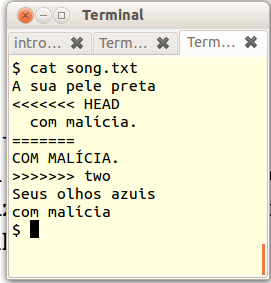
\includegraphics[width=60.0mm]{merge-conflict.eps}
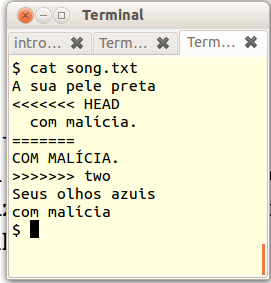
\includegraphics[width=\linewidth]{merge-conflict.eps}
%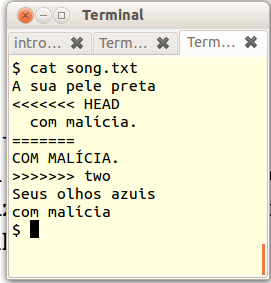
\includegraphics[width=5cm]{merge-conflict.png}
        \end{column}
\end{columns}
\end{frame}

% ---------------------------------------------------------------------
\begin{frame}[fragile]
\frametitle{Merging - Conflicts}

\CMD{\$git config -{}-global merge.tool vimdiff}

\vspace{.1\textheight}

\CMD{\$ git mergetool}
\begin{Verbatim}[commandchars=\\\{\}]
Merging:
song.txt

Normal merge conflict for 'song.txt':
  {local}: modified file
  {remote}: modified file
Hit return to start merge resolution tool (vimdiff):
\end{Verbatim}

\end{frame}

% ---------------------------------------------------------------------
\begin{frame}[fragile]
\frametitle{Merging - Conflicts}

\begin{center}
%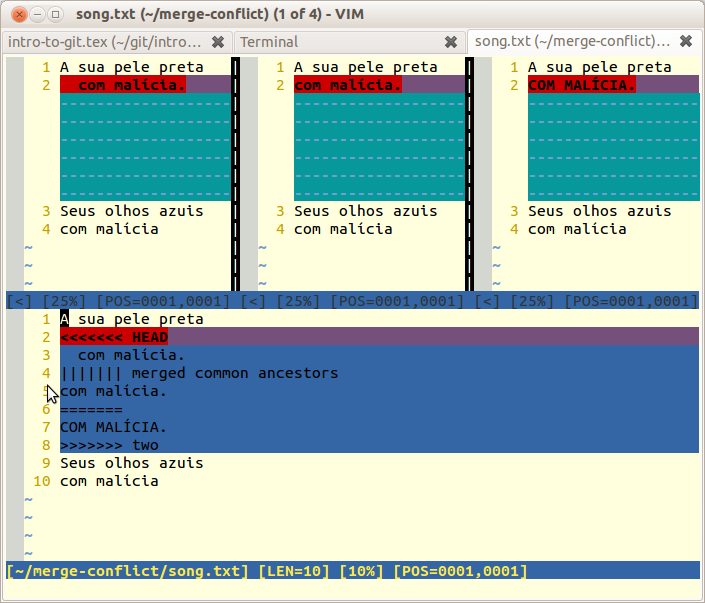
\includegraphics[width=60.0mm]{merge-tool.eps}
\includegraphics[width=\linewidth]{merge-tool.eps}
%\includegraphics[width=5cm]{merge-tool.png}
\end{center}

\end{frame}

% =====================================================================
\mysubsection{Remotes}{using:remotes}

% ---------------------------------------------------------------------
\begin{frame}
\frametitle{Decentralization}
\includegraphics[width=0.5\linewidth]{cloning-1-upstream.eps}
\begin{itemize}
        \item public repository
\end{itemize}
\end{frame}

% ---------------------------------------------------------------------
\begin{frame}
\frametitle{Decentralization}
\includegraphics[width=0.5\linewidth]{cloning-2-local.eps}
\begin{itemize}
        \item make a local clone
\end{itemize}
\end{frame}

% ---------------------------------------------------------------------
\begin{frame}
\frametitle{Decentralization}
\includegraphics[width=0.5\linewidth]{cloning-3-topic.eps}
\begin{itemize}
        \item local cloning is lighweight
\end{itemize}
\end{frame}

% ---------------------------------------------------------------------
\begin{frame}
\frametitle{Decentralization}
\includegraphics[width=0.5\linewidth]{cloning-4-push.eps}
\begin{itemize}
        \item push changes between any repositories
\end{itemize}
\end{frame}

% ---------------------------------------------------------------------
\begin{frame}
\frametitle{Decentralization}
\includegraphics[width=0.5\linewidth]{cloning-5-publish.eps}
\begin{itemize}
        \item publish changes to public server
\end{itemize}
\end{frame}

% ---------------------------------------------------------------------
\begin{frame}
\frametitle{Decentralization}
\includegraphics[width=0.7\linewidth]{cloning-6-trusted.eps}
\begin{itemize}
        \item share changes with trusted peers
\end{itemize}
\end{frame}

% ---------------------------------------------------------------------
\begin{frame}
\frametitle{Is Decentralization any good?}

\begin{itemize}
        \item non-intrusive micro-commits
        \item detached operation
        \item no single point of failure
        \item backups are trivial
\end{itemize}
\end{frame}

% ---------------------------------------------------------------------
\begin{frame}
\frametitle{Cloning}

\CMD{\$ git clone <remote>} \\
\begin{itemize}
        \item replicates \green{remote} repository
        \item populates new repository
        \item checks out new working tree
\end{itemize}
\end{frame}

% ---------------------------------------------------------------------
\begin{frame}[fragile]
\frametitle{Git URLs}

\begin{itemize}
        \item local repo \\
                \begin{Verbatim}[commandchars=\\\{\}]
\CMD{/home/git/project.git/}
\CMD{file:///home/git/project.git/}
                \end{Verbatim}
                \vspace{\baselineskip}


        \item http protocol \\
                \begin{Verbatim}[commandchars=\\\{\}]
\CMD{http://repo.or.cz/r/git.git}
                \end{Verbatim}
                \vspace{\baselineskip}


        \item native git protocol
                \begin{Verbatim}[commandchars=\\\{\}]
\CMD{git://repo.or.cz/git.git}
                \end{Verbatim}
                \vspace{\baselineskip}


        \item ssh protocol
                \begin{Verbatim}[commandchars=\\\{\}]
\CMD{ssh://bart@jukie.net/~git/project.git/}
\CMD{bart@jukie.net/~git/project.git/}
                \end{Verbatim}
\end{itemize}
\end{frame}

% ---------------------------------------------------------------------
\begin{frame}[fragile]
\frametitle{Working with remotes}

\includegraphics[width=0.6\linewidth]{remote-12.eps}

\begin{center}
        \CMD{git fetch} + \CMD{git merge}


        =

        \CMD{git pull}
\end{center}
\vspace{\textheight}
\end{frame}

% ---------------------------------------------------------------------
\begin{frame}
\frametitle{Working with remotes}

\begin{itemize}
        \item bare vs normal repos
        \item pushing
        \item creating \\
\CMD{\$ git clone -{}-bare} \\
\end{itemize}

\end{frame}

% ---------------------------------------------------------------------
\begin{frame}[fragile]
\frametitle{Working with remotes}

\includegraphics[width=0.6\linewidth]{remote-16.eps}

\begin{Verbatim}[commandchars=\\\{\}]
\CMD{\$ git push}
\end{Verbatim}
\vspace{\textheight}
\end{frame}

% ---------------------------------------------------------------------
\begin{frame}[fragile]
\frametitle{Working with remotes}

\includegraphics[width=0.9\linewidth]{remote-24.eps}

\CMD{\$ git remote add fred http://foo.com/project.git/}
\vspace{\textheight}
\end{frame}

% ---------------------------------------------------------------------
\begin{frame}[fragile]
\frametitle{Working with remotes}

\includegraphics[width=0.9\linewidth]{remote-29.eps}

\begin{Verbatim}[commandchars=\\\{\}]
\CMD{\$ git log \red{fred/master}}
\end{Verbatim}

\vspace{\textheight}
\end{frame}

% ---------------------------------------------------------------------
\begin{frame}[fragile]
\frametitle{Working with remotes}

\includegraphics[width=0.9\linewidth]{remote-29.eps}

\begin{Verbatim}[commandchars=\\\{\}]
\CMD{\$ git checkout -b fred-fix \red{fred/master}}
\end{Verbatim}

\vspace{\textheight}
\end{frame}

% ---------------------------------------------------------------------
\begin{frame}[fragile]
\frametitle{Working with remotes}

\includegraphics[width=0.9\linewidth]{remote-31.eps}

\begin{Verbatim}[commandchars=\\\{\}]
\CMD{\$ git checkout master}
\end{Verbatim}

\vspace{\textheight}
\end{frame}

% ---------------------------------------------------------------------
\begin{frame}[fragile]
\frametitle{Working with remotes}

\includegraphics[width=0.9\linewidth]{remote-32.eps}

\begin{Verbatim}[commandchars=\\\{\}]
\fnt{\$ git checkout master}
\CMD{\$ git merge fred-fix}
\end{Verbatim}

\vspace{\textheight}
\end{frame}

% ---------------------------------------------------------------------
\begin{frame}[fragile]
\frametitle{Working with remotes}

\includegraphics[width=0.9\linewidth]{remote-33.eps}

\begin{Verbatim}[commandchars=\\\{\}]
\fnt{\$ git checkout master}
\fnt{\$ git merge fred-fix}
\CMD{\$ git branch -d fred-fix}
\end{Verbatim}

\vspace{\textheight}
\end{frame}

% ---------------------------------------------------------------------
\begin{frame}[fragile]
\frametitle{Working with remotes}

\includegraphics[width=0.9\linewidth]{remote-34.eps}

\begin{center}
\CMD{\$ git push}
\end{center}

\vspace{\textheight}
\end{frame}

% ---------------------------------------------------------------------
\begin{frame}[fragile]
\frametitle{Working with remotes}

\includegraphics[width=0.9\linewidth]{remote-37.eps}

\vspace{\textheight}
\end{frame}

% ---------------------------------------------------------------------
\begin{frame}[fragile]
\frametitle{Working with remotes}

Scenario:
\begin{itemize}
        \item laptop - normal repo
        \item want a bare repo, somewhere else \\
        \item rsync?
\end{itemize}

\end{frame}

% ---------------------------------------------------------------------
\begin{frame}[fragile]
\frametitle{Working with remotes}

\CMD{remote\$ git init -{}-bare} \\
\vspace{.1\textheight}
\CMD{local\$ git remote add foo ...} \\
\CMD{local\$ git push foo master}

\end{frame}

% ---------------------------------------------------------------------
\begin{frame}[fragile]
\frametitle{Working with remotes}

Scenario:
\begin{itemize}
        \item 2 laptops - normal repos
        \item want to push between them
\end{itemize}

\end{frame}

% ---------------------------------------------------------------------
\begin{frame}[fragile]
\frametitle{Working with remotes}

\CMD{local\$ git remote add foo ...} \\
\CMD{local\$ git push foo master:dummy} \\
\vspace{.1\textheight}
\CMD{remote\$ git checkout target} \\
\CMD{remote\$ git merge dummy} \\
\CMD{remote\$ git branch -d dummy} \\

\end{frame}

% =====================================================================
\mysubsection{Rebasing}{using:rebasing}
% ---------------------------------------------------------------------
\begin{frame}
\frametitle{Rebasing}

\begin{itemize}
        \item in existing branch
        \vspace{.1\textheight}
        \item from a different branch
\end{itemize}
\end{frame}

% ---------------------------------------------------------------------
\begin{frame}
\frametitle{Rebasing}

\begin{itemize}
        \item you're rewriting history
        \item Warning! Warning! Danger, Will Robinson!
\end{itemize}
\end{frame}

% ---------------------------------------------------------------------
\begin{frame}
\frametitle{Rebasing - Existing Branch}

\CMD{\$ git rebase -i HEAD tilda 7}
\begin{itemize}
        \item start rebase
\end{itemize}

\vspace{.05\textheight}
\CMD{\$ git reset HEAD caret} \\
\CMD{\$ git add -p} \\
\CMD{\$ git commit -{}-amend}
\begin{itemize}
        \item do edits
\end{itemize}

\vspace{.05\textheight}
\CMD{\$ git rebase -{}-continue}
\begin{itemize}
        \item keep going
\end{itemize}

\vspace{.05\textheight}
\CMD{\$ git rebase -{}-abort}
\begin{itemize}
        \item made a mistake, start again...
\end{itemize}

\end{frame}

% ---------------------------------------------------------------------
\begin{frame}
\frametitle{Rebasing - Different Branch}

\CMD{\$ git rebase <branch>} \\
\begin{itemize}
        \item moves new work onto a new baseline
        \item can cause \red{conflicts} \\
                \faint{ie: require user intervention}
\end{itemize}
\end{frame}

% ---------------------------------------------------------------------
\begin{frame}
\frametitle{Rebasing - Different Branch}

\includegraphics[width=\linewidth]{branch-vs-rebase-01.eps}
\vspace{\baselineskip}
\begin{center}
        take two identical trees
\end{center}
\vspace{\textheight}
\end{frame}

% ---------------------------------------------------------------------
\begin{frame}
\frametitle{Rebasing - Different Branch}

\includegraphics[width=\linewidth]{branch-vs-rebase-02.eps}
\vspace{\baselineskip}
\begin{flushleft}
        \CMD{\$ git merge master}
\end{flushleft}
\vspace{\textheight}
\end{frame}

% ---------------------------------------------------------------------
\begin{frame}
\frametitle{Rebasing - Different Branch}

\includegraphics[width=\linewidth]{branch-vs-rebase-03.eps}
\vspace{\baselineskip}
\begin{center}
        that's easy
\end{center}
\vspace{\textheight}
\end{frame}

% ---------------------------------------------------------------------
\begin{frame}
\frametitle{Rebasing - Different Branch}

\includegraphics[width=\linewidth]{branch-vs-rebase-03.eps}
\vspace{\baselineskip}
\begin{flushright}
        \CMD{\$ git rebase master}
\end{flushright}
\vspace{\textheight}
\end{frame}

% ---------------------------------------------------------------------
\begin{frame}
\frametitle{Rebasing - Different Branch}

\includegraphics[width=\linewidth]{branch-vs-rebase-04.eps}
\vspace{\baselineskip}
\begin{flushright}
        \CMD{\$ git rebase master}
\end{flushright}
\vspace{\textheight}
\end{frame}

% ---------------------------------------------------------------------
\begin{frame}
\frametitle{Rebasing - Different Branch}

\includegraphics[width=\linewidth]{branch-vs-rebase-05.eps}
\vspace{\baselineskip}
\begin{flushright}
        \CMD{\$ git rebase master}
\end{flushright}
\vspace{\textheight}
\end{frame}

% ---------------------------------------------------------------------
\begin{frame}
\frametitle{Rebasing - Different Branch}

\includegraphics[width=\linewidth]{branch-vs-rebase-06.eps}
\vspace{\baselineskip}
\begin{flushright}
        \CMD{\$ git rebase master}
\end{flushright}
\vspace{\textheight}
\end{frame}

% ---------------------------------------------------------------------
\begin{frame}
\frametitle{Rebasing - Different Branch}

\includegraphics[width=\linewidth]{branch-vs-rebase-07.eps}
\vspace{\baselineskip}
\begin{flushright}
        \CMD{\$ git rebase master}
\end{flushright}
\vspace{\textheight}
\end{frame}

% ---------------------------------------------------------------------
\begin{frame}
\frametitle{Rebasing - Different Branch}

\includegraphics[width=\linewidth]{branch-vs-rebase-08.eps}
\vspace{\baselineskip}
\begin{flushright}
        \CMD{\$ git rebase master}
\end{flushright}
\vspace{\textheight}
\end{frame}

% ---------------------------------------------------------------------
\begin{frame}
\frametitle{Rebasing - Different Branch}

\includegraphics[width=\linewidth]{branch-vs-rebase-09.eps}
\vspace{\baselineskip}
\begin{flushright}
        \CMD{\$ git rebase master}
\end{flushright}
\vspace{\textheight}
\end{frame}

% ---------------------------------------------------------------------
\begin{frame}
\frametitle{Rebasing - Different Branch}

\includegraphics[width=\linewidth]{branch-vs-rebase-10.eps}
\vspace{\baselineskip}
\begin{flushright}
        \CMD{\$ git rebase master}
\end{flushright}
\vspace{\textheight}
\end{frame}

% ---------------------------------------------------------------------
\begin{frame}
\frametitle{Rebasing - Different Branch}

\includegraphics[width=\linewidth]{branch-vs-rebase-11.eps}
\vspace{\textheight}
\end{frame}

% ---------------------------------------------------------------------
\begin{frame}
\frametitle{Rebasing vs Cherrypicking}

\begin{columns}[t]
        \begin{column}[T]{.5\textwidth}
                you're on 'wicked' \\
                \vspace{\baselineskip}
                want 'C' into 'wicked'
        \end{column}
        \begin{column}[T]{.5\textwidth}
                \includegraphics[width=\linewidth]{branching-12.eps}
        \end{column}
\end{columns}
\vspace{.05\textheight}
\CMD{\$ git cherry-pick 45b2d8}
\end{frame}

% =====================================================================
\mysubsection{Inspection}{using:inspection}
% ---------------------------------------------------------------------
\begin{frame}
\frametitle{Object references}

specific commit ID\ldots
\vspace{\baselineskip}

{\small
\begin{tabular}{ll}
        full hash      & \ttt{6bb1270ffb60cbfef87266d2d4b4abe4218d9c68} \\
        short hash     & \ttt{6bb127} \\
        & \\
        tag            & \textcolor{blue}{v1.5.6.1} \\
        local branch   & \textcolor{green}{master} \\
        remote branch  & \textcolor{red}{origin/master} \\
        & \\
        by message     & ``:/some text'' \\
        & \\
        checkout       & HEAD \\
        last fetch     & FETCH\_HEAD \\
        previous head  & ORIG\_HEAD \\
        \ldots & \\
\end{tabular}
}

\vspace{.1\textheight}

\end{frame}

% ---------------------------------------------------------------------
\begin{frame}
\frametitle{Why? Diffs, Logs}

\CMD{\$ git diff \$commit \$commit}
\begin{itemize}
        \item changes between two commits
\end{itemize}

\end{frame}

% ---------------------------------------------------------------------
\begin{frame}[fragile]
\frametitle{Object references}

a commit before HEAD

\vspace{.1\textheight}
\begin{center}
        \faint{HEAD}\verb!^   ==   ! \faint{HEAD}\verb!~!1
\end{center}

\end{frame}

% ---------------------------------------------------------------------
\begin{frame}[fragile]
\frametitle{Object references}

few commits before HEAD

\vspace{.1\textheight}
\begin{center}
        \faint{HEAD}\verb!^^^   ==   ! \faint{HEAD}\verb!~!3
\end{center}

\end{frame}

% ---------------------------------------------------------------------
\begin{frame}[fragile]
\frametitle{Object references}

few commits before master

\vspace{.1\textheight}
\begin{center}
        \faint{master}\verb!^^^   ==   ! \faint{master}\verb!~!3
\end{center}

\end{frame}

% ---------------------------------------------------------------------
\begin{frame}[fragile]
\frametitle{Object references}

what was it yesterday?

\vspace{.1\textheight}
\begin{center}
        @\{yesterday\} \verb!   ==   ! \faint{HEAD}@\{yesterday\}
\end{center}

\end{frame}

% ---------------------------------------------------------------------
\begin{frame}
\frametitle{Object references}

how about my-other-branch on June 1st?

\vspace{.1\textheight}
\begin{center}
        \faint{my-other-branch}@\{June.1\}
\end{center}

\end{frame}

% ---------------------------------------------------------------------
\begin{frame}
\frametitle{Object references}

master a few changes ago?

\vspace{.1\textheight}
\begin{center}
        \faint{master}@\{3\}
\end{center}

\end{frame}

% ---------------------------------------------------------------------
\begin{frame}[fragile]
\frametitle{Show me!}

review last commit\ldots
\vspace{\baselineskip}

\CMD{\$ git show}
{\small
\begin{Verbatim}[commandchars=\\\{\}]
\textcolor{brown}{commit 83b2d051814e884a8e264127ed47552a5dcf6c1d}
Author: Bart Trojanowski <bart@jukie.net>
Date:   Thu Jul 3 21:44:39 2008 -0400

    changed one line

diff --git a/test b/test
index 808a2c4..99810fa 100644
--- a/test
+++ b/test
\textcolor{cyan}{@@ -1,3 +1,3 @@}
 Some old text before the change.
\textcolor{red}{-Some text for removal.}
\textcolor{green}{+Replacement line.}
 Some old text after the change.
\end{Verbatim}
}
\vspace{\textheight}
\end{frame}

% ---------------------------------------------------------------------
\begin{frame}[fragile]
\frametitle{Show me!}

just the stats\ldots
\vspace{\baselineskip}

\CMD{\$ git show {-}-stat}
{\small
\begin{Verbatim}[commandchars=\\\{\}]
\textcolor{brown}{commit 83b2d051814e884a8e264127ed47552a5dcf6c1d}
Author: Bart Trojanowski <bart@jukie.net>
Date:   Thu Jul 3 21:44:39 2008 -0400

    changed one line

 test |    2 \textcolor{green}{+}\textcolor{red}{-}
 1 files changed, 1 insertions(+), 1 deletions(-)
\end{Verbatim}
}
\vspace{\textheight}
\end{frame}

% ---------------------------------------------------------------------
\begin{frame}[fragile]
\frametitle{Show me!}

SVN'esq status information\ldots
\vspace{\baselineskip}

\CMD{\$ git show {-}-name-status}
{\small
\begin{Verbatim}[commandchars=\\\{\}]
\textcolor{brown}{commit 3d3d2989b817af3fd4fa6d63f200113bd6c94bdb}
Author: Bart Trojanowski <bart@jukie.net>
Date:   Thu Jul 3 22:59:13 2008 -0400

    something more interesting

A       sub/bar
D       sub/foo
M       test
\end{Verbatim}
}
\vspace{\textheight}
\end{frame}

% ---------------------------------------------------------------------
\begin{frame}[fragile]
\frametitle{Show me!}

review any other commit\ldots
\vspace{\baselineskip}

\begin{Verbatim}[commandchars=\\\{\}]
\CMD{\$ git show HEAD}
\CMD{\$ git show HEAD^^^}
\CMD{\$ git show master\Verb!~10!}
\CMD{\$ git show master@\{May.16\}}
\end{Verbatim}

\ldots

\vspace{\textheight}
\end{frame}

% ---------------------------------------------------------------------
\begin{frame}[fragile]
\frametitle{Show me!}

show a file (or tree) in history\ldots
\vspace{\baselineskip}

\CMD{\$ git show HEAD:file}
{\small
\begin{Verbatim}[commandchars=\\\{\}]
contents\ldots
\end{Verbatim}
}
\vspace{\textheight}
\end{frame}

% ---------------------------------------------------------------------
\begin{frame}[fragile]
\frametitle{Logs}

See commit history\ldots
\vspace{\baselineskip}

\CMD{\$ git log}
{\tiny
\begin{Verbatim}[commandchars=\\\{\}]
\textcolor{brown}{commit 3d3d2989b817af3fd4fa6d63f200113bd6c94bdb}
Author: Bart Trojanowski <bart@jukie.net>
Date:   Thu Jul 3 22:59:13 2008 -0400

    most recent commit

\textcolor{brown}{commit 83b2d051814e884a8e264127ed47552a5dcf6c1d}
Author: Bart Trojanowski <bart@jukie.net>
Date:   Thu Jul 3 21:44:39 2008 -0400

    second most recent

\textcolor{brown}{commit 1cc1b35a611c39f49842e2ca28d40886c1ae9b7c}
Author: Bart Trojanowski <bart@jukie.net>
Date:   Thu Jul 3 21:44:05 2008 -0400

    middle commit

\textcolor{brown}{commit 411515f51a78d66a27a7d56ebe9f70dbd2bff008}
Author: Bart Trojanowski <bart@jukie.net>
Date:   Thu Jul 3 21:43:36 2008 -0400

    second oldest

\textcolor{brown}{commit 52a0ff44aba8599f43a5d821c421af316cb73051}
Author: Bart Trojanowski <bart@jukie.net>
Date:   Mon Jun 30 21:44:55 2008 -0400

    oldest commit

\end{Verbatim}
}
\ldots
\vspace{\textheight}
\end{frame}

% ---------------------------------------------------------------------
\begin{frame}[fragile]
\frametitle{Logs}

limit by range\ldots
\vspace{\baselineskip}

\begin{Verbatim}[commandchars=\\\{\}]
\CMD{\$ git log tag..branch}
\CMD{\$ git log HEAD~10..}
\CMD{\$ git log branch1 branch2 ^common}

\CMD{\$ git log -10}
\CMD{\$ git log -10 master@\{yesterday\}}

\CMD{\$ git log {-}-since="May 1" {-}-until="June 1"}
\end{Verbatim}

\vspace{\textheight}
\end{frame}

% ---------------------------------------------------------------------
\begin{frame}[fragile]
\frametitle{Logs}

limit by commit attributes\ldots
\vspace{\baselineskip}

\begin{Verbatim}[commandchars=\\\{\}]
\CMD{\$ git log {-}-author=fred}
\CMD{\$ git log {-}-committer=joe}
\CMD{\$ git log {-}-grep="commit.*message.*text"}
\end{Verbatim}

\vspace{\textheight}
\end{frame}

% ---------------------------------------------------------------------
\begin{frame}[fragile]
\frametitle{Logs}

search for a change\ldots
\vspace{\baselineskip}

\begin{Verbatim}[commandchars=\\\{\}]
\CMD{\$ git log -S"some code change"}
\CMD{\$ git log {-}-pickaxe-regex -S"some.*code.*change"}
\end{Verbatim}

\vspace{\textheight}
\end{frame}

% ---------------------------------------------------------------------
\begin{frame}[fragile]
\frametitle{Logs}

limit by changes to specific path\ldots
\vspace{\baselineskip}

\begin{Verbatim}[commandchars=\\\{\}]
\CMD{\$ git log -- some/file}
\end{Verbatim}

\vspace{\textheight}
\end{frame}

% ---------------------------------------------------------------------
\begin{frame}[fragile]
\frametitle{Faster grep}

another way to search\ldots
\vspace{\baselineskip}

\begin{Verbatim}[commandchars=\\\{\}]
\CMD{\$ git grep -e "pattern" -- some/file}


\vspace{\baselineskip}
\CMD{\$ git grep -e "pattern" branch -- some/file}
\end{Verbatim}

\vspace{\textheight}
\end{frame}

% =====================================================================
\mysubsection{Further Reading}{using:end}
% ---------------------------------------------------------------------
\begin{frame}
\frametitle{Further reading}
\begin{center}
        \blue{Git Magic} \\
        \blue{GitCasts.com} \faint{(Scott Chacon)} \\
        \blue{GitHub.com} \\
\end{center}
\end{frame}

% =====================================================================
% vim: set makeprg=make:
\end{document}
